% ****************************************************************************************************
\chapter[Business Models of Platform as a Service Providers -- Current State]{Business Models of Platform as a Service\protect\linebreak Providers -- Current State}\label{ch:sota}
% ****************************************************************************************************

In order to assess the current state of \ac{PaaS} providers' business models and identify their key elements, the current business models of 23 \ac{PaaS} providers were analyzed. The initial selection of the \ac{PaaS} providers analyzed in this thesis was based on technical reports and market reports provided by three different market research companies:
\begin{itemize}[parsep=0pt, topsep=0pt, itemsep=0pt]
	\item Forrester Research, Inc. -- \citet{Rymer2011,Ried2011a}
	\item \ac{IDC} -- \citet{Bradshaw2012,Hendrick2012, Hendrick2012a}
	\item Gartner, Inc. -- \citet{Smith2012}
\end{itemize}
The \ac{PaaS} providers initially identified and selected were further whittled down to receive a manageable set of representative \ac{PaaS} providers. Four disjunct selection criteria were used in the second evaluation round to identify the final set of 23 \ac{PaaS} providers, viz. (1) market share, (2) growth rate, (3) availability of the platform to customers as of February 2013, and (4) background of the \ac{PaaS} provider, for instance, formerly purely \ac{IaaS} or \ac{SaaS} providers extending their cloud portfolio with \ac{PaaS} functionalities. According to \citet{Hendrick2012}, the world largest \ac{PaaS} provider is GXS Worldwide, Inc. (cf. Appendix \ref{ch:app01:gxs}) with a market share of 14.2\% in 2011. With a growth rate of 428.6\% in 2011, CloudBees is the fastest-growing \ac{PaaS} provider (cf. Subsection \ref{ch:sota:cb}).

In the first part of this chapter detailed descriptions of four representative case studies are given, i.e. CloudBees, GigaSpaces Cloudify, Facebook Developers, and SAP HANA Cloud. To obtain a coherent representation, all the business models investigated in this thesis follow the approach to business model conceptualization introduced previously (cf. Subsection \ref{ch:tf:bmc}). The remaining 19 case studies are presented in Appendix \ref{ch:app01} for reasons of comprehensibility. All 23 cases studies are based on data available as of February 2013. Based upon the performed analysis of these \ac{PaaS} providers' current business models, a classification scheme for \ac{PaaS} providers was developed, which is introduced in Section \ref{ch:sota:cm}. At the end of this chapter, this classification scheme is used to give an overview of the selected \ac{PaaS} providers, followed by a short dicussion.

%In the first part of this chapter four case studies -- CloudBees, GigaSpaces Cloudify, Facebook Developers, and SAP Hana Cloud -- are described representatively in detail. The remaining 19 case studies are presented for reasons of comprehensibility within Appendix \ref{ch:app01}. All 23 presented cases studies are based on data available as of February 2013. To receive a coherent representation, all presented business models within this thesis follow the prior introduced business model conceptualization approach (cf. Subsection \ref{ch:sota:bmc}). Based upon the performed analyzes of current \ac{PaaS} providers' business models, a classification scheme for \ac{PaaS} providers was developed and is introduced in Section \ref{ch:sota:cm}. At the end of this chapter an overview of all investigated \ac{PaaS} providers by the use of the developed classification scheme is provided as well as shortly discussed.

\section{Representative Case Studies}

The main focus in conducting these case studies was on how these business models appear on the market and are experienced by their customers, rather than how they are implemented by a specific company or how they are viewed internally. For this reason, the market view elements, i.e. the \ac{CVP} and, in parts, the profit formula, are mainly considered, even though the non-market view elements, i.e. key resources and key processes, are mentioned whenever possible. Moreover, focusing on market view elements allowed to solely utilize secondary data for the analysis of \ac{PaaS} providers' business models, for instance reliable, public data or documentation, both providing comprehensive information about the business model under investigation. Information concerning the internal business model elements, viz. key resources, key processes, and, in parts, the profit formula, is difficult to obtain due to the fact that this information is kept confidential in most cases, e.g. the cost structure as well as process or workflow descriptions. Thus, the following presented business models mainly focus on the market view elements.

\subsection{CloudBees}\label{ch:sota:cb}

CloudBees was founded in the beginning of 2012 and soon introduced its identically named \ac{PaaS} offer. Many members of the CloudBees' management team, including the founder, had previously worked for companies like Oracle, Sun, IBM, and VMware or were involved in development projects around JBoss and Jenkins CI. The background of CloudBees' management already reveals the main objective -- a \ac{PaaS} solution specifically designed for the Java programming language ecosystem, supporting the whole application lifecycle \citep{CloudBees2013}. The CloudBees platform is composed of two distinct but related elements. First, all development, integration, and testing tasks are performed within the DEV@cloud. The core of this part of the platform is the Jenkins Continuous Integration server. Once an application is ready to go live, the application is migrated to the RUN@cloud. Basically, the RUN@cloud represents a traditional application server, including the functionalities load balancing, scalability, and high availability, based on various cloud infrastructures.

CloudBees platform solution mainly attracts two different customer groups: business end-consumers and \acp{ISV}. The first group utilizes the platform to manage the entire application lifecycle, including development, quality assurance and testing, deployment and release management, as well as monitoring and administration. Due to the fact that all applications upon the CloudBees platform are based on standard Java and not on specific CloudBees \acp{API}, potential customers are not faced with a so-called lock-in effect. Moreover, platform customers can select between multi-tenant and individual RUN@clouds. In the case of individual instances, they can choose the appropriate cloud infrastructure. Private, public, and hybrid provisioning scenarios are supported. Via the CloudBees Partner Ecosystem, business end-consumers can purchase third-party applications and services and extend the CloudBees platform functionalities. 

Platform extensions are provided by the second customer group, the \acp{ISV}. CloudBees's uniquely defined mission is to support the whole application lifecycle for standard Java and \ac{JVM} based applications within the cloud, which enables \acp{ISV} to expand the already existing platform capabilities by deploying and testing tools, comprehensive monitoring features, as well as different databases. All third-party applications, tools, and services are listed in the CloudBees Partner Ecosystem. Especially small \acp{ISV}, but certainly also all other \acp{ISV}, greatly benefit from the fact, that payments including billing for third-party extensions is handled by CloudBees.

The overall revenue of CloudBees is composed of two revenue streams: on the one hand, CloudBees' partners, and on the other its platform customers. Consulting partners, i.e. \acp{SI}, need to pay an annual partner fee (currently 2.000 \ac{USD} for silver partners and 5.000 \ac{USD} for gold partners) to become a certified CloudBees Service Partner. For all third-party applications, tools, and services provided by \acp{ISV} (which CloudBees calls as Technology Partners), CloudBees gets a default revenue share of 30\%. However, CloudBees also offers the possibility to negotiate the revenue share rate individually.

Business end-consumers pay a combination of subscription and transaction based fees for the CloudBees platform. The DEV@cloud is available in four different packages: Free (0 \ac{USD} per month), Base (15 \ac{USD}), Pro (50 \ac{USD}), and Enterprise (100 \ac{USD}). Each offer includes different features and quotas, as well as a different number of build minutes. Additional build minutes can be purchased for 0.106 \ac{USD} or 0.425 \ac{USD} per hour, depending on the package. A multi-tenant RUN@cloud is either free (no additional features or services can be purchased) or charged per hour, based on the select application server and SSL connections. As mentioned above, the dedicated RUN@cloud can basically be hosted at any cloud infrastructure, meaning that a vast number of pricing models is possible. For instance, the CloudBees RUN@cloud platform hosted at \ac{AWS} infrastructure is priced between 153 - 644 \ac{USD} per instance monthly. Furthermore, CloudBees is offering also a MySQL database which is priced based on the selected RUN@cloud \citep{CloudBees2013}. An illustration of the above business model can be found in Table \ref{bm:cloudbees}:

% ****************************************************************************************************
% Business Model CloudBees NEW
% ****************************************************************************************************
\begin{longtable}{L{\column}L{\column}L{\column}L{\column}}
	
	\caption[Business Model CloudBees]{Business Model CloudBees \citep{CloudBees2013}}
	\label{bm:cloudbees}\\
	
	\toprule
	\multicolumn{4}{l}{\small \textit{\nameref{bm:cloudbees}}}\\ 
	\midrule
	\endfirsthead
	\toprule  
	\multicolumn{4}{l}{\small \textit{continued from previous page (\nameref{bm:cloudbees})}}\\ 
	\midrule
	\endhead
	\multicolumn{4}{r}{\small \textit{continued on next page}}\\
	\bottomrule
	\endfoot
	\bottomrule
	\endlastfoot
	
	\multicolumn{4}{c}{\small \textbf{Customer Value Proposition (CVP)}}\\ \midrule
	
	\small Target customer &
	\small Job to be done &
	\multicolumn{2}{L{\columnT}}{\small Offering} \\ \midrule
	
	% START CUSTOMERS
	\small
	Business End-Consumer &
	\small
	Manage the entire Java application lifecycle within the cloud in a cost efficiency manner & 
	\multicolumn{2}{L{\columnT}}{
	\vspace{-5mm}
	\small
	\begin{itemize}[leftmargin=*, parsep=0pt, topsep=0pt, itemsep=0pt]
				\item Manage the entire Java and \ac{JVM} application lifecycle
				\item CloudBees Eclipse plugin and \ac{SDK}
				\item Different deployment scenarios: public, private, and hybrid
				\item 'No vendor lock-in' (standard Java)
				\item CloudBees partner ecosystem provides platform extensions -- databases, monitoring as well as deployment tools\vspace{-\baselineskip} 
		\end{itemize}
	} \\ \midrule
	\small	
	\ac{ISV} &
	\small
	Develop, manage, and market application lifecycle related applications and services globally &
	\multicolumn{2}{L{\columnT}}{
		\vspace{-5mm} 
		\small
		\begin{itemize}[leftmargin=*, parsep=0pt, topsep=0pt, itemsep=0pt]
				\item CloudBees platform as a service truly dedicated to Java and \ac{JVM} applications (clear mission)
				\item Service resp. application listing within the Ecosystem Technology Partner directory
				\item Support mechanism between CloudBees and service provider, to resolve customer problems within a narrow time frame
				\item Joint marketing activities
				\item Payment handling (incl. billing) by CloudBees\vspace{-\baselineskip} 
		\end{itemize}
	} \\ \midrule

% END CUSTOMERS

% KEY RESOURCES
\multicolumn{2}{L{\columnT}}{ \textbf{Key Resources}
\small
\begin{itemize}[leftmargin=*, parsep=0pt, topsep=0pt, itemsep=0pt]
				\item CloudBees' platform, including
					\begin{itemize}[leftmargin=*, topsep=0pt, itemsep=0pt]
						\item Build: create, integrate, and test
						\item Run: choose, deploy, and store
						\item Manage: scale, monitor, and enhance
					\end{itemize}
				\item CloudBees Eclipse plugin and \ac{SDK}
				\item Consulting partners, for instance Black Diamond Software
				\item Partnership with \ac{IaaS} providers, for instance \ac{AWS}\vspace{-\baselineskip} 
	\end{itemize}
} &
% KEY PPROCESSES
\multicolumn{2}{L{\columnT}}{ \textbf{Key Processes}
\small
\begin{itemize}[leftmargin=*, parsep=0pt, topsep=0pt, itemsep=0pt]
				\item Maintain full lifecycle support for Java and \ac{JVM} applications as well as keep the platform up to date (in respect of new Java versions and features)
				\item Facilitate different deployment scenarios -- public, private, and hybrid -- based on multiple \ac{IaaS} providers
				\item Maintain partnerships with existing \ac{IaaS} providers as well as begin negotiations with potential providers
				\item Partner program for consulting partners, including business and marketing support, access to products plans, trainings, reselling options, and listing in the CloudBees Service Partner Directory
				\item Offer support via Stack Overflow, \ac{FAQ}, and documentation/ guides deployment tools\vspace{-\baselineskip} 
\end{itemize}
} \\ \midrule

% PROFIT FORMULA
\multicolumn{4}{L{\columnF}}{ \textbf{Profit Formula}
	\small
	\begin{itemize}[leftmargin=*, parsep=0pt, topsep=0pt, itemsep=0pt]
				\item Subscription and transaction based revenue for platform usage:
					\begin{itemize}[leftmargin=*, topsep=0pt, itemsep=0pt]
						\item DEV@cloud: USD 0 - 100 / Monthly + build minutes
						\item RUN@cloud Multi-Tenant: Free (limited) or transaction based (depends among other things on the used software stack per app per hour) 
						\item RUN@cloud Dedicated: Different IaaS providers, e.g. \ac{AWS} US m1.small USD 153 \/ Monthly
						\item Database: Offered by CloudBees (MySQL) USD 0 - 25 / Monthly or by different partners
					\end{itemize}
				\item Partner program fee: USD 2000 - 5000 / Yearly
				\item Revenue sharing (30\%; or individual negotiated) for applications and services offered by third parties\vspace{-\baselineskip} 
	\end{itemize}
} \\

\end{longtable}





\subsection{GigaSpaces Cloudify}\label{ch:sota:gsc}

Within the evolving \ac{PaaS} ecosystem just a few open source platform solutions are available -- Cloudify is one of them. The Cloudify Open \ac{PaaS} Stack has been available on the market since the beginning of 2012. Cloudify itself and the Cloudify Community are promoted by the company GigaSpaces \citep{GigaSpaces2013a}.

The basic concept of Cloudify is the so-called external blueprint, also called the recipe. Within a blueprint the deployment and post-deployment activities of an application are described. This concept enables developers to migrate existing applications to cloud infrastructure without the need to adopt or change the source code. Moreover, based on the blueprint concept, applications can be deployed at or migrated between private, public, or even hybrid cloud infrastructures \citep{GigaSpaces2013a}.

Two distinct customer groups can use the Cloudify platform offer: (1) business end-consumers who want to move existing non-cloud applications to the cloud or develop and operate cloud applications and (2) \acp{ISV} who want to offer migration services (migrate on-premise applications onto cloud infrastructure). The value proposition for these two stakeholder groups include the promise to move any application without changes in the code or application architecture to the cloud, to develop a one-time external blueprint for an application and be able to deploy the application at different cloud infrastructures, as well as to gain full control over the Cloudify Open \ac{PaaS} Stack. Furthermore, an interactive shell and web-based user interface for monitoring purposes are provided \citep{GigaSpaces2013a}.

As is usual for many open source projects, a flourishing community, in this case the Cloudify Community, actively participates around the open source product. Within the Cloudify Community, product-related knowledge is shared via support forums, documentations, events, blogs, and videos. Moreover, the Cloudify platform source code and sample Cloudify blueprints and recipes are publicly available via GitHub \citep{GigaSpaces2013b,GitHub2013,GitHub2013a}.

GigaSpaces' Cloudify platform is offered as an open source platform, meaning the platform software itself is free of charge. However, it should be noted that Cloudify platform users still need the corresponding cloud infrastructure, which is offered for a fee, e.g. by \ac{AWS}, Rackspace, and HPCloud. Various fee-based services for Cloudify are provided by GigaSpaces, including technical support, training, and consultancy services \citep{GigaSpaces2013a}. An illustration of this business model is presented in Table \ref{bm:cloudify}:

% ****************************************************************************************************
% Business Model GigaSpaces Cloudify NEW
% ****************************************************************************************************
\begin{longtable}{L{\column}L{\column}L{\column}L{\column}}
	
	\caption[Business Model GigaSpaces Cloudify]{Business Model GigaSpaces Cloudify \citep{GigaSpaces2013a,GigaSpaces2013b}}
	\label{bm:cloudify}\\
	
	\toprule
	\multicolumn{4}{l}{\footnotesize \textit{\nameref{bm:cloudify}}}\\ 
	\midrule
	\endfirsthead
	\toprule
	\multicolumn{4}{l}{\footnotesize \textit{continued from previous page (\nameref{bm:cloudify})}}\\ 
	\midrule
	\endhead
	\multicolumn{4}{r}{\footnotesize \textit{continued on next page}}\\
	\bottomrule
	\endfoot
	\bottomrule
	\endlastfoot
	
	\multicolumn{4}{c}{\small \textbf{Customer Value Proposition (CVP)}}\\ \midrule

	\footnotesize Target customer &
	\footnotesize Job to be done &
	\multicolumn{2}{L{\columnT}}{\footnotesize Offering} \\ \midrule
	
	% START CUSTOMERS
	
	\footnotesize 
	Business End-Consumer &
	\footnotesize 
	Operate applications in the cloud  & 
	
	\multicolumn{2}{L{\columnT}}{
	\vspace{-5mm} 
		\footnotesize 
		\begin{itemize}[leftmargin=*, parsep=0pt, topsep=0pt, itemsep=0pt]
				\item Move any application (without code changes) to the cloud
				\item 'No vendor lock-in' (no specific programming language)
				\item Deployment and post-deployment steps (installing, starting, orchestrating, and monitoring) are described within a blueprint (also known as recipe)\vspace{-\baselineskip} 
		\end{itemize}
	}\\ \midrule
	
	\footnotesize 
	\ac{ISV} &
	\footnotesize 
	Offer migration services (on-premise onto cloud infrastructure) to customers & 
	\multicolumn{2}{L{\columnT}}{
	\vspace{-5mm} 
		\footnotesize 
		\begin{itemize}[leftmargin=*, parsep=0pt, topsep=0pt, itemsep=0pt]
				\item Different deployment scenarios: public, private, and hybrid; fast migration process through blueprint concept
				\item Local testing 
				\item Full control over the platform stack
				\item Automatic scaling based on custom metrics (scale-in and scale-out)
				\item Cloudify shell \vspace{-\baselineskip} 
		\end{itemize}
	}	\\ \midrule

% END CUSTOMERS

% KEY RESOURCES
\multicolumn{2}{L{\columnT}}{\small \textbf{Key Resources}
	\footnotesize 
	\begin{itemize}[leftmargin=*, parsep=0pt, topsep=0pt, itemsep=0pt]
				\item Open source Cloudify platform stack
				\item Cloudify Community
				\item Blueprint resp. recipe concept
				\item Cloud Driver \ac{API}
				\item Web-based user-interface (monitoring)
				\item Cloudify shell\vspace{-\baselineskip} 
	\end{itemize}
} &
% KEY PPROCESSES
\multicolumn{2}{L{\columnT}}{\small \textbf{Key Processes}
	\footnotesize 
	\begin{itemize}[leftmargin=*, parsep=0pt, topsep=0pt, itemsep=0pt]
				\item Maintain, improve, and extend the blueprint/ recipe concept, the Cloud Driver \ac{API}, as well as the web-based user interface
				\item Provide instructions how to build or ready to use blueprints/ recipes, for instance how to deploy a multi-tier application on \ac{AWS} infrastructure
				\item Promote the Cloudify Community\vspace{-\baselineskip} 
	\end{itemize}
} \\ \midrule

% PROFIT FORMULA
\multicolumn{4}{L{\columnF}}{\small \textbf{Profit Formula}
	\footnotesize 
	\begin{itemize}[leftmargin=*, parsep=0pt, topsep=0pt, itemsep=0pt]
		\item \ac{OSS}
		\item Various charged services provided by GigaSpaces:
		\begin{itemize}[leftmargin=*, parsep=0pt, topsep=0pt, itemsep=0pt]
			\item Technical support
			\item Account and product management
			\item Education services
			\item Consultancy services for Cloudify: on-boarding support, assessments and reviews, as well as implementation projects\vspace{-\baselineskip} 
		\end{itemize}
	\end{itemize}
} \\

\end{longtable}





\subsection{Facebook Developers}\label{ch:sota:fd}

Facebook, the social network with more than a billion monthly active users, 655 million daily active users, and 751 million monthly active users using mobile devices to access Facebook's social network (all figures as of March 2013), introduced its \ac{PaaS} offer, called Facebook Developers, in May 2007 \citep{Facebook2013}. By the end of March 2012, more than nine million applications and websites had been built directly upon the Facebook Developers platform or by utilizing features of it, which were then integrated with Facebook \citep{Facebook2013}. Facebook Developers derives its attractiveness especially from Facebook's large user base,  providing millions of potential users of applications and websites.

The Facebook Developers platform can be used to integrate Facebook features and services with (mobile) applications as well as websites. On the other hand, the platform can also be used to integrate (mobile) applications with Facebook. Furthermore, advertisers provide advertisement services which can be used by developers to monetize their efforts. The Facebook Developers platform provides a comprehensive set of tools and features to support different kinds of development and administrative tasks \citep{Facebook2013a} such as Facebook \acp{SDK} for iOS, Android, JavaScript, and PHP; third-party \acp{API} for .NET (C\#), Falsh (ActionScript), Python, Java (Spring), Java (BlackBerry), Ruby, and Node.js; Facebook \acp{API} like Login, Graph \ac{API}, and Facebook Query Language (FQL); and tools like the Graph \ac{API} Explorer as well as a JavaScript Test Console. Applications are distributed over the Facebook App Center (marketplace) with linkage functionality for native mobile applications, e.g. for iOS applications linkage to the App Store, and for Android applications linkage to the Google Play Store; as well as on-demand provisioning for non-native mobile or browser-based applications.

Facebook is generating monetary revenue mainly through the following three revenue streams. First, new or already existing applications can be promoted through a fee-based advertising self-service. Facebook offers the possibility of defining the target audience, e.g. by region, age, or gender, the promoting goal, e.g. getting installs, and the budget of the ad campaign. Second, application users can purchase digital and virtual goods in social applications based on the currency Facebook Credits. Since the end of 2012, the option of local currency pricing has also been offered \citep{Facebook2013a}. In order to use in-app payment, users need to buy Facebook Credits or, in the case of local currency pricing, pay directly with their credit card, PayPal, or another payment method. On the other hand, the application or service provider can exchange the Facebook Credits obtained through their applications and services for real money. Facebook retains a 30\% charge for this service. And third, most likely the most important revenue stream is generated through personalized advertisements, for instance within applications and websites.

Furthermore, Facebook also generates non-monetary revenue by capturing valuable user data in more detail. It is possible to log in to various websites and services (built with the help of features of the Facebook Developer platform) with a valid Facebook account -- a kind of single sign-on (SSO) system which can be considered a lock-in effect and allows Facebook to collect valuable user data from various external sources. An illustration of this business model is given in Table \ref{bm:facebook}:

\newpage
% ****************************************************************************************************
% Business Model Facebook Developers
% ****************************************************************************************************
\begin{longtable}{L{\column}L{\column}L{\column}L{\column}}
	
	\caption[Business Model Facebook Developers]{Business Model Facebook Developers \citep{Facebook2013a,Facebook2013}}
	\label{bm:facebook}\\
	
	\toprule
	\multicolumn{4}{l}{\textit{\nameref{bm:facebook}}}\\ 
	\midrule
	\endfirsthead
	\toprule  
	\multicolumn{4}{l}{\textit{continued from previous page (\nameref{bm:facebook})}}\\ 
	\midrule
	\endhead
	\multicolumn{4}{r}{\textit{continued on next page}}\\
	\bottomrule
	\endfoot
	\bottomrule
	\endlastfoot
	
	\multicolumn{4}{c}{ \textbf{Customer Value Proposition (CVP)}}\\ \midrule
	
	Target customer &
	Job to be done &
	\multicolumn{2}{L{\columnT}}{Offering} \\ \midrule
	
	% START CUSTOMERS
	\small
	\ac{ISV} &
	\small
	Develop and market browser as well as mobile applications resp. games & 
	\multicolumn{2}{L{\columnT}}{
	\vspace{-5mm}
	\small
	\begin{itemize}[leftmargin=*, parsep=0pt, topsep=0pt, itemsep=0pt]
				\item Facebook and third-party \acp{SDK}
				\item Facebook \acp{API}
				\item Income through advertisements and Facebook Credits
				\item Tools like the JavaScript Test Console
				\item Service for free
				\item Existing user base\vspace{-\baselineskip} 
		\end{itemize}
	} \\ \midrule
	\small	
	Business End-Consumer &
	\small
	Integrate social network services into (existing) applications and websites &
	\multicolumn{2}{L{\columnT}}{
		\vspace{-5mm} 
		\small
		\begin{itemize}[leftmargin=*, parsep=0pt, topsep=0pt, itemsep=0pt]
				\item Facebook and third-party \acp{SDK}
				\item Facebook \acp{API}
				\item Social Plugins
				\item Tools like the JavaScript Test Console
				\item Service for free
				\item Existing user base\vspace{-\baselineskip} 
		\end{itemize}
	} \\ \midrule
	\small	
	Advertising Broker &
	\small
	Act as an intermediary between advertisers and developers resp. application providers &
	\multicolumn{2}{L{\columnT}}{
		\vspace{-5mm} 
		\small
		\begin{itemize}[leftmargin=*, parsep=0pt, topsep=0pt, itemsep=0pt]
				\item Flourishing global ecosystem with broad user base
				\item Certification process for advertising providers
				\item Public list with all approved advertising providers\vspace{-\baselineskip} 
		\end{itemize}
	} \\ \midrule
	\small	
	Private End-Consumer &
	\small
	Participation in a social network including diverse games resp. applications &
	\multicolumn{2}{L{\columnT}}{
		\vspace{-5mm} 
		\small
		\begin{itemize}[leftmargin=*, parsep=0pt, topsep=0pt, itemsep=0pt]
				\item Facebook.com
				\item Facebook App Center
				\item Social plugins\vspace{-\baselineskip} 
		\end{itemize}
	} \\ \midrule

% END CUSTOMERS

% KEY RESOURCES
\multicolumn{2}{L{\columnT}}{ \textbf{Key Resources}
\small
\begin{itemize}[leftmargin=*, parsep=0pt, topsep=0pt, itemsep=0pt]
				\item Infrastructure
				\item Facebook.com
				\item Existing user base
				\item Facebook \acp{SDK} for iOS, Android, JavaScript, and PHP (provided by Facebook itself)
				\item Third-party \acp{SDK} for .NET (C\#), Flash (ActionScript), Python, Java (Spring), Java (BlackBerry), Ruby, and Node.js
				\item Facebook \acp{API}: Login, Graph \ac{API}, Facebook Query Language (FQL), and Ads \ac{API}
				\item Facebook App Center (marketplace) with linkage (for native applications) as well as provisioning (browser-based applications)
				\item Social Plugins: Link Button, Follow Button, Login Button and more
				\item Tools: Graph \ac{API} Explorer, JavaScript Test Console, and more\vspace{-\baselineskip} 
	\end{itemize}
} &
% KEY PPROCESSES
\multicolumn{2}{L{\columnT}}{ \textbf{Key Processes}
\small
\begin{itemize}[leftmargin=*, parsep=0pt, topsep=0pt, itemsep=0pt]
				\item Infrastructure management
				\item Linkage management between Facebook App Center and Google Play Store as well as Apple App Store
				\item Payment services for Facebook Credits: purchase (mainly by application users) and exchange (mainly by application providers)
				\item Partner program, i.e. Preferred Marketing Developer Program
				\item Maintain and publish documentations, sample applications, and best practices
				\item Offer support via Stack Overflow, Facebook Communities, and \ac{FAQ}
\vspace{-\baselineskip} 
\end{itemize}
} \\ \midrule

% PROFIT FORMULA
\multicolumn{4}{L{\columnF}}{ \textbf{Profit Formula}
	\small
	\begin{itemize}[leftmargin=*, parsep=0pt, topsep=0pt, itemsep=0pt]
				\item Monetary:
					\begin{itemize}[leftmargin=*, topsep=0pt, itemsep=0pt]
						\item Promoting service for new applications
						\item Facebook credit (also local currency pricing):
Possible use case: An application user buys equipment paid by Facebook Credits within a game. The application provider changes these credits into real money -- Facebook takes a 30\% charge.
						\item Personalized advertisements
					\end{itemize}
				\item Non-Monetary:
				\begin{itemize}[leftmargin=*, topsep=0pt, itemsep=0pt]
						\item Detailed and valuable user data
					\end{itemize}\vspace{-\baselineskip} 
	\end{itemize}
} \\

\end{longtable}





\subsection{SAP HANA Cloud}\label{ch:sota:sap}

SAP, a German enterprise software vendor with more than 200.000 customers worldwide, launched a new \ac{PaaS} solution named SAP HANA Cloud at the end of 2012 \citep{SAP2013b,SAP2013a}. SAP HANA Cloud aims to support the development, deployment, and management of stand-alone as well as integrated cloud applications. The platform itself and the applications built upon the platform are both hosted by SAP with a guaranteed system availability of 99.9\% \citep{SAP2013b}.

SAP's new \ac{PaaS} solution is targeting four diverse stakeholder groups. Application customers who want to use pure \ac{SaaS} applications, as well as to complement existing SAP and non-SAP on-premise systems with cloud applications, represent the first customer group. Presumably the most important part of SAP's offering for this stakeholder group, is the SAP Store with certified third-party applications (including quality assurance) and the guaranteed system availability of 99.9\%.

Development partners, which constitute the second stakeholder group, utilize the platform to develop, deploy, manage, and market business \ac{SaaS} applications globally. SAP's existing installed base, comprising more than 200.000 customers, worldwide represent potential customers for business applications built upon SAP HANA Cloud. Due to the fact that the applications are built with the programming language Java, SAP provides an Eclipse plugin as well as a corresponding \ac{SDK}. Thus, developers are able to develop applications within the well-known and open \ac{IDE} Eclipse as well as test and debug applications locally. Furthermore, various capabilities of integration with SAP and non-SAP on-premise systems are provided or are currently under development. In addition, all applications can use SAP HANA, SAP's in-memory database technology. Further offerings for development partners include the SAP Store as channel, comprehensive support services, and best practice sharing with regard to application pricing.

The third stakeholder group is comprised of the so-called platform customers. These customers subscribe and use the SAP HANA Cloud platform to be able to react continuously to internal and to market demands in a cost-efficient manner. In most cases, these customers maintain their own internal \ac{IT} department, which develops business cloud applications integrable with SAP and non-SAP on premise systems. The offering for this group includes the Eclipse plugin and \ac{SDK}, the integration capabilities, access to SAP HANA, the SAP Store to purchase third-party applications, support services, as well as the \ac{SLA} concerning the system availability.

Finally, SAP offers an Individual Developer License to the fourth stakeholder group: the individual developers. This free yet non-productive license allows developers to get access to the SAP HANA Cloud platform and to experience as well as test the platform capabilities. Obviously, the offering for individual developers include the Eclipse plugin and corresponding \ac{SDK} as well as various support services, like tutorials and sample applications, all in sense of the objective to keep the entry barriers as low as possible. SAP aims for these individual developers to feel confident with the SAP HANA Cloud platform capabilities, and to decide to participate as development partners in the ecosystem in the near future.

The revenue for SAP is based on the following revenue streams: As mentioned above, the SAP HANA Cloud platform itself can be subscribed to by customers as a whole. Most likely these customers are upper \acp{SME} or large enterprises. Subscriptions to the platform come as pre-defined packages, including certain quotas for structured and unstructured storage, bandwidth, connections to SAP and non-SAP on-premise systems, as well as computing units. Currently, four different packages are available \citep{SAP2013b}: (1) Individual Developer License for free, (2) Starter Package (370 \ac{EUR}), (3) Professional Package (4.800 \ac{EUR}), and (4) Premium Package (16.000 \ac{EUR}). Furthermore, customers can also compile their own package, based on the following six metrics: (1) virtual machines, (2) unstructured storage (e.g. documents), (3) structured storage (HANA), (4) structured storage (\ac{RDBMS}), (5) bandwidth, and (6) connections to third-party systems (SAP systems are free). 

\acp{ISV}, startup companies, and solution providers, subsumed under the term development partners, provide applications upon the SAP HANA Cloud platform \citep{SAP2013a}. In order to utilize SAP's platform, development partners need to pay an annual partner fee of 1.990 \ac{EUR}. All third-party applications available within the SAP Store are certified by SAP. Application providers need to pay an initial application certification fee (990 \ac{EUR}) and recurring annual fees (495 \ac{EUR}). Furthermore, SAP gets a 15\% revenue share (offset against the annual partner fee) for all applications based on SAP HANA Cloud and sold via the SAP Store. Table \ref{bm:sap} illustrates the above business model:

% ****************************************************************************************************
% Business Model SAP Hana Cloud NEW
% ****************************************************************************************************
\begin{longtable}{L{\column}L{\column}L{\column}L{\column}}
	
	\caption[Business Model SAP HANA Cloud]{Business Model SAP HANA Cloud \citep{SAP2013b,SAP2013a}}
	\label{bm:sap}\\
	
	\toprule
	\multicolumn{4}{l}{\footnotesize \textit{\nameref{bm:sap}}}\\ 
	\midrule
	\endfirsthead
	\toprule
	\multicolumn{4}{l}{\footnotesize \textit{continued from previous page (\nameref{bm:sap})}}\\ 
	\midrule
	\endhead
	\multicolumn{4}{r}{\footnotesize \textit{continued on next page}}\\
	\bottomrule
	\endfoot
	\bottomrule
	\endlastfoot
	
	\multicolumn{4}{c}{\small \textbf{Customer Value Proposition (CVP)}}\\ \midrule
	
	\footnotesize Target customer &
	\footnotesize Job to be done &
	\multicolumn{2}{L{\columnT}}{\footnotesize Offering} \\ \midrule
	
	% START CUSTOMERS
	\footnotesize 
	App Customers &
	\footnotesize 
	Use or complement on-premise systems with \ac{SaaS} applications & 
	\multicolumn{2}{L{\columnT}}{
	\vspace{-5mm}
	\footnotesize 
	\begin{itemize}[leftmargin=*, parsep=0pt, topsep=0pt, itemsep=0pt]
				\item SAP Store as channel
				\item Certified applications in the SAP Store (quality assurance by SAP)
				\item Trusted Brand
				\item Leverage prior investments in SAP, non-SAP, and legacy systems through possibilities for integration
				\item Hosted by SAP (platform) with a guaranteed availability of 99.9\% (via \ac{SLA})\vspace{-\baselineskip} 
		\end{itemize}
	} \\ \midrule
	\footnotesize 	
	Development Partners (\acp{ISV} and System Integrators) &
	\footnotesize 
	Develop, deploy, manage, and market business \ac{SaaS} applications globally &
	\multicolumn{2}{L{\columnT}}{
		\vspace{-5mm} 
		\footnotesize 
		\begin{itemize}[leftmargin=*, parsep=0pt, topsep=0pt, itemsep=0pt]
				\item SAP HANA Cloud Eclipse plugin and \ac{SDK} (Java)
				\item Various possibilities for integration
				\item Installed base/ customer base
				\item SAP Store as channel
				\item Revenue share rate of 15\%
				\item SAP HANA inside (in-memory database technology)
				\item Platform is hosted by SAP with a guaranteed availability of 99.9\% (via \ac{SLA})
				\item Support via SAP Community Network, \ac{FAQ}, and documentation/ guides
				\item Best practices regarding application pricing\vspace{-\baselineskip} 
		\end{itemize}
	} \\ \midrule
	\footnotesize 	
	Platform Customers (large enterprises and upper \acp{SME}) &
	\footnotesize 
	React continuously to internal and market demands in a cost-efficient manner and develop business applications, integrable with legacy and SAP systems
 &
	\multicolumn{2}{L{\columnT}}{
		\vspace{-5mm} 
		\footnotesize 
		\begin{itemize}[leftmargin=*, parsep=0pt, topsep=0pt, itemsep=0pt]
				\item SAP HANA Cloud Eclipse plugin and \ac{SDK} (Java)
				\item Various possibilities for integration
				\item SAP HANA inside (in-memory database technology)
				\item Platform is hosted by SAP with a guaranteed availability of 99.9\% (via \ac{SLA})
				\item Trusted brand
				\item Enterprise readiness (SLAs, downtime)
				\item SAP Store
				\item Support via SAP Community Network, \ac{FAQ}, and documentation/ guides\vspace{-\baselineskip} 
		\end{itemize}
	} \\ \midrule
	\footnotesize 	
	Individual Developers &
	\footnotesize 
	Develop applications with standard tools (low entry barrier) &
	\multicolumn{2}{L{\columnT}}{
		\vspace{-5mm} 
		\footnotesize 
		\begin{itemize}[leftmargin=*, parsep=0pt, topsep=0pt, itemsep=0pt]
				\item Free developer license (non-productive system)
				\item SAP HANA Cloud Eclipse plugin and \ac{SDK} (Java)
				\item Support via SAP Community Network, \ac{FAQ}, and documentation/ guides
				\item SAP HANA inside (in-memory database technology)\vspace{-\baselineskip} 
		\end{itemize}
	} \\ \midrule

% END CUSTOMERS

% KEY RESOURCES
\multicolumn{2}{L{\columnT}}{\small \textbf{Key Resources}
\footnotesize 
\begin{itemize}[leftmargin=*, parsep=0pt, topsep=0pt, itemsep=0pt]
				\item Infrastructure (data center) for hosting the SAP HANA Cloud platform as well as the \ac{SaaS} applications offered via the SAP Store
				\item SAP HANA Cloud platform
				\item SAP HANA Cloud Eclipse plugin and \ac{SDK}
				\item Brand (SAP)
				\item SAP Store
				\item Planned sales partners
				\item Platform technology partners: providing complementing platform features (for instance Mail Service)\vspace{-\baselineskip} 
	\end{itemize}
} &
% KEY PPROCESSES
\multicolumn{2}{L{\columnT}}{\small \textbf{Key Processes}
\footnotesize 
\begin{itemize}[leftmargin=*, parsep=0pt, topsep=0pt, itemsep=0pt]
				\item Infrastructure management: 24/7 reliable services, globally available to fulfill the guaranteed availability of 99.9\% 
				\item Efficient operations
				\item Partner management
				\item Efficient and rapid certification process for applications
				\item Providing possibilities for integration for all SAP applications
				\item Efficient low cost sales channel (e.g. self-service)
				\item Offering support via SAP Community Network, \ac{FAQ}, and documentation/ guides\vspace{-\baselineskip} 
\end{itemize}
} \\ \midrule

% PROFIT FORMULA
\multicolumn{4}{L{\columnF}}{\small \textbf{Profit Formula}
	\footnotesize 
	\begin{itemize}[leftmargin=*, parsep=0pt, topsep=0pt, itemsep=0pt]
				\item Platform subscription:
					\begin{itemize}[leftmargin=*, topsep=0pt, itemsep=0pt]
						\item SAP HANA Cloud packages: \ac{EUR} 370 - 16.000 / Month or
						\item Individually composed packages based on six metrics: virtual machine, unstructured storage (i.e. documents), structured storage (HANA and RDBMS), bandwidth, and connections to third party systems (SAP systems are free)
					\end{itemize}
				\item Annual fee for development partners: \ac{EUR} 1.990 
				\item Revenue sharing (15\%) for applications provided via the SAP Store (offset against annual partner fee)
				\item Application certification fee: initially \ac{EUR} 990, then \ac{EUR} 495 per year
				\item Infrastructure and development costs
				\item Sales and marketing (direct channel) costs\vspace{-\baselineskip} 
	\end{itemize}
} \\

\end{longtable}





\section{Classification Scheme}\label{ch:sota:cm}

\textit{"Classification is an important tool for perception, because it provides clarity. \ldots\xspace Well-known examples are the periodic table of the elements in chemistry \ldots\xspace and the decimal classification in library science"} \citep[p. 36]{Fettke2003}. In order to achieve this objective, the classification methodology introduced by \citet{Fettke2003} is used to develop a classification scheme for \ac{PaaS} business models. This classification scheme will facilitate the comparison of \ac{PaaS} business models and will be considered along with the business model conceptualization by \citet{Johnson2008}, where the latter supports the representation of business models and as such relies on the classification scheme. According to \citet[p. 39]{Fettke2003}, \textit{"a classification scheme consists of a set of characteristics which are suitable to classify objects of a specific application domain"}. Within each classification process, the crucial step is to select the appropriate classification objects and characteristics, neither too general nor too specific. The following six universal guidelines are helpful to improve the quality of classification schemes: completeness, precision, consistency, extensibility, user-friendliness, and economic efficiency \citep[pp. 40-41]{Fettke2003}. 

Five interrelated phases which are performed subsequently, and possibly iteratively, constitute the proposed classification methodology (cf. Figure \ref{fig:cm}): (1) inception, (2) elaborate characteristics, (3) specify classification scheme, (4) test, and (5) use and maintenance. These five phases were applied as follows:

\begin{enumerate}
	\item Inception: For the purpose of classifying \ac{PaaS} business models, a corresponding classification scheme was needed. This scheme should further serve as a starting point for the interdependencies within \ac{PaaS} business models introduced later (cf. Chapter \ref{ch:cld}).

	\item Elaborate characteristics: The data obtained through the comprehensive analysis of existing \ac{PaaS} business models was analyzed on the one hand in terms of stand-alone business models, i.e. analyzing within-case data, and on the other hand to search for cross-case patterns \citep[pp. 539-540]{Eisenhardt1989}. In the process of identifying potential cross-case patterns, two different approaches were used. First, the four elements of the business model representation (cf. Section \ref{ch:tf:bmc}) introduced by \citet{Johnson2008} were used to compare business models and reveal similarities as well as fundamental differences. Second, pairs of business models were selected and compared to uncover further potentially distinguishing features. 

	\item Specify classification scheme: In order to connect the identified \ac{PaaS} business model criteria as well as their characteristics in a structured approach, the concept of a morphological matrix adapted from \citet{ Zwicky1969} was used, as depicted in Figure \ref{fig:cs}. This classification scheme enables to classify \ac{PaaS} business models, and hence constitutes the solution of the first sub-research question.

	\item Test: By classify the set of 23 \ac{PaaS} business models chosen for investigation, the classification scheme was evaluated and iteratively revised as well as enhanced, where classify is considered \textit{"an operation whereby objects \ldots\xspace are assigned to classes \ldots\xspace which have been previously defined"} \citep[p. 130]{Marradi1990}.

	\item Use and maintenance: The \ac{PaaS} business model classification scheme (cf. Figure \ref{fig:cs}) finally obtained was used to survey the business models of 23 \ac{PaaS} providers (cf. Section \ref{ch:sota:cPaaS}) and as a basis to answer the second sub-research question (cf. Chapter \ref{ch:cld}).
\end{enumerate}

\begin{figure}[t]
	\centering
	% ****************************************************************************************************
% Classification Procedural Model
% ****************************************************************************************************

\begin{tikzpicture}[scale=0.75, every node/.style={scale=0.75}]

\node[draw,text width=7em,text centered,rectangle,rounded corners,minimum height=4em,thick] (1) at (5,5.5) {(1) Inception};
\node[draw,text width=7em,text centered,rectangle,rounded corners,minimum height=4em,thick] (2) at (9,3) {(2) Elaborate Characteristics};
\node[draw,text width=7em,text centered,rectangle,rounded corners,minimum height=4em,thick] (3) at (8,0) {(3) Specify Classification Scheme};
\node[draw,text width=7em,text centered,rectangle,rounded corners,minimum height=4em,thick] (4) at (2,0) {(4) Test};
\node[draw,text width=7em,text centered,rectangle,rounded corners,minimum height=4em,thick] (5) at (1,3) {(5) Use and Maintenance};

\node[align=left,font=\small] (t1) at (11,5.5) {
	\begin{minipage}{4.7cm}
		\begin{itemize}[leftmargin=*, parsep=0pt, topsep=0pt, itemsep=0pt]
			\item Basic Conditions of Classification
			\item Preliminary Decisions of Classification Principle
			\item Index of Sources
		\end{itemize}
	\end{minipage}
};

\node[align=left,font=\small] (t2) at (11.5,1.2) {
	\begin{minipage}{4cm}
		\begin{itemize}[leftmargin=*, parsep=0pt, topsep=0pt, itemsep=0pt]
			\item Set of Characteristics
			\item Frequency Scale of Characteristics
		\end{itemize}
	\end{minipage}
};

\node[align=left,font=\small] (t3) at (5.4,-1.25) {
	\begin{minipage}{5cm}
		\begin{itemize}[leftmargin=*, parsep=0pt, topsep=0pt, itemsep=0pt]
			\item Classification Scheme
		\end{itemize}
	\end{minipage}
};

\node[align=left,font=\small] (t4) at (-1,1.5) {
	\begin{minipage}{4cm}
		\begin{itemize}[leftmargin=*, parsep=0pt, topsep=0pt, itemsep=0pt]
			\item Tested Classification Scheme
		\end{itemize}
	\end{minipage}
};

\node[align=left,font=\small] (t5) at (2,5) {
	\begin{minipage}{5cm}
		\begin{itemize}[leftmargin=*, parsep=0pt, topsep=0pt, itemsep=0pt]
			\item Shortcomings
			\item Revisions
		\end{itemize}
	\end{minipage}
};


\path 
	(1.east) edge [->,thick,>=stealth'] (2.north)
	(2.south) edge [->,thick,>=stealth'] (3.north)
	(3.west) edge [->,thick,>=stealth'] (4.east)
	(4.north) edge [->,thick,>=stealth'] (5.south)
	(5.north) edge [->,thick,>=stealth'] (1.west);

\end{tikzpicture}
	\caption[Classification Methodology]{Classification Methodology, adapted from \citet[p. 44]{Fettke2003}}
	\label{fig:cm}
\end{figure}

The classification scheme for \ac{PaaS} business models which finally resulted (cf. Figure \ref{fig:cs}) consists of five classification criteria (first column) and the cardinality of each classification criterion\footnote{A cardinality of $n$ means that a \ac{PaaS} business model can comprise several characteristics of the corresponding classification criterion, whereas a cardinality of $1$ implies a singular classification criterion.} (second column). Hereafter the characteristics of each classification criterion are mentioned. Five essential classification criteria have been identified, viz. (1) customer segment, (2) core value proposition, (3) governance model, (4) technical scope, and (5) revenue stream. These criteria as well as the characteristics were revealed by using case study techniques according to \citet{Eisenhardt1989} and \citet{Yin2008}. The overall process is known as multi-case, multi-unit case study research \citep{Yin2008} and the units of investigation were derived from the literature (\citealp{Johnson2008} and \citealp{Tiwana2010}) and through evidence. By using the approach of a cross-case pattern search according to \citet{Eisenhardt1989} in combination with \citet{Johnson2008} business model conceptualization, three criteria were derived. First, the criterion 'customer segment' was deduced from the business model element \ac{CVP}, in particular from the part 'target customer'. Also, the second criterion, 'core value proposition', was based on this element; here the offering was the main reason. And finally, the criterion 'revenue stream' was derived from the business model element 'profit formula'. The remaining two criteria, i.e. 'governance model' and 'technical scope',  were deduced by comparing business models in pairs, where these criteria can partly be ascribed to the two business model elements 'key resources' and 'key processes'. Possible differences in the governance model are in alignment with \citet{Tiwana2010}. During the process of analysis of the case studies the diversity of technical capabilities was remarkable.

The first criterion 'customer segment' consists of five characteristics which were found in the 23 investigated \ac{PaaS} business models --  (1) \ac{IT} startup, (2) \ac{SI}, (3) \ac{ISV}, (4) platform customer, and (5) application customer. \ac{PaaS} providers try to reach and serve these groups of people or companies in order to operate a profitable business. In most cases, \ac{IT} startups are dynamic in their early stages and thus will use new technologies and products earlier than established companies. For example, the SAP HANA Cloud platform tries to attract \ac{IT} startups through a free developer license so as to provide low entry barriers. These early adaptors will thereby help to place the platform within the market. \acp{SI} provide complementing services, for instance consulting services. Through a dedicated \ac{CVP} especially for \acp{SI}, Dell aims to convince this group of customers to offer services for their platform Dell Boomi. Platform extensions and custom developments are provided by \acp{ISV}. By offering low revenue share rates, for instance Salesfore.com Force.com with 15\% and 25\% respectively, and SAP HANA Cloud with 15\%, platform providers attempt to be attractive for this customer group. In general, \ac{PaaS} platforms serve two different end customer groups. On the one hand, platform customers use the platform internally to develop new applications and services (e.g. the platforms GXS Trading Grid and OrangeScape Cloud) and, on the other hand, application customers purchase applications built upon the platform and distributed through a marketplace (for instance the platforms Caspio Bridge and NetSuite SuiteCloud).

\begin{figure}[tb]
	\centering
	% ****************************************************************************************************
% Classification Scheme
% ****************************************************************************************************

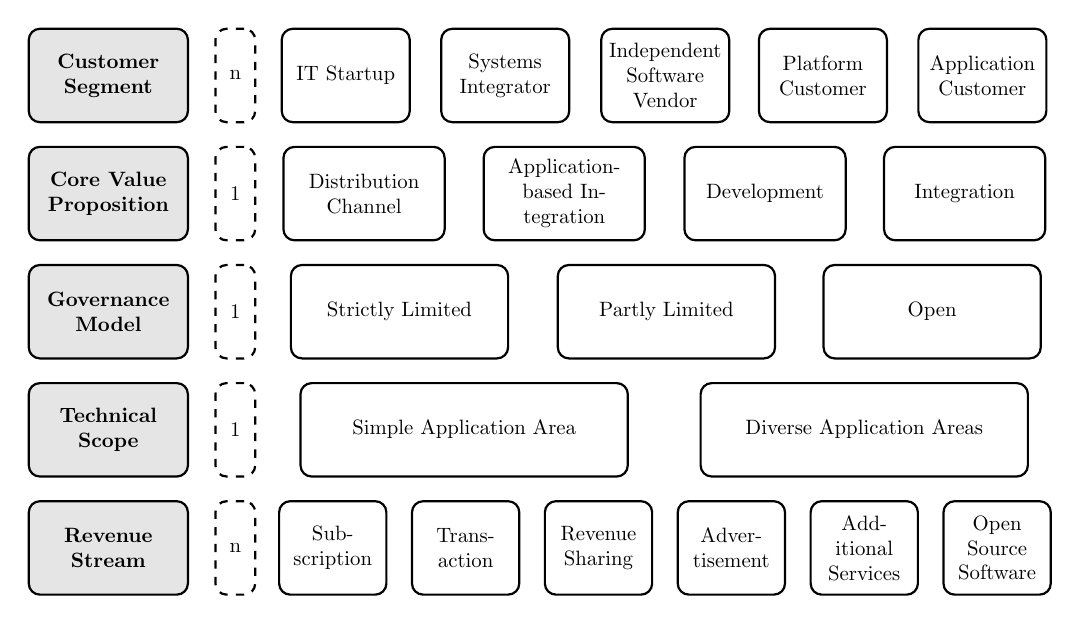
\begin{tikzpicture}[scale=0.75, every node/.style={scale=0.75}]

\node[font={\bfseries},draw,text width=7em,text centered,rectangle,rounded corners,minimum height=4.5em,thick,fill=gray!20] (1) at (-1,8) {Customer Segment};
\node[font={\bfseries},draw,text width=7em,text centered,rectangle,rounded corners,minimum height=4.5em,thick,fill=gray!20] (1) at (-1,6) {Core Value Proposition};
\node[font={\bfseries},draw,text width=7em,text centered,rectangle,rounded corners,minimum height=4.5em,thick,fill=gray!20] (1) at (-1,4) {Governance Model};
\node[font={\bfseries},draw,text width=7em,text centered,rectangle,rounded corners,minimum height=4.5em,thick,fill=gray!20] (1) at (-1,2) {Technical Scope};
\node[font={\bfseries},draw,text width=7em,text centered,rectangle,rounded corners,minimum height=4.5em,thick,fill=gray!20] (1) at (-1,0) {Revenue Stream};

\node[draw,text width=1.25em,text centered,rectangle,rounded corners,minimum height=4.5em,thick,dashed] (1) at (1.15,8) {n};
\node[draw,text width=1.25em,text centered,rectangle,rounded corners,minimum height=4.5em,thick,dashed] (1) at (1.15,6) {1};
\node[draw,text width=1.25em,text centered,rectangle,rounded corners,minimum height=4.5em,thick,dashed] (1) at (1.15,4) {1};
\node[draw,text width=1.25em,text centered,rectangle,rounded corners,minimum height=4.5em,thick,dashed] (1) at (1.15,2) {1};
\node[draw,text width=1.25em,text centered,rectangle,rounded corners,minimum height=4.5em,thick,dashed] (1) at (1.15,0) {n};




\node[draw,text width=5.5em,text centered,rectangle,rounded corners,minimum height=4.5em,thick] (1) at (3.02,8) {IT Startup};
\node[draw,text width=5.5em,text centered,rectangle,rounded corners,minimum height=4.5em,thick] (1) at (5.72,8) {Systems Integrator};
\node[draw,text width=5.5em,text centered,rectangle,rounded corners,minimum height=4.5em,thick] (1) at (8.43,8) {Independent Software Vendor};
\node[draw,text width=5.5em,text centered,rectangle,rounded corners,minimum height=4.5em,thick] (1) at (11.1,8) {Platform Customer};
\node[draw,text width=5.5em,text centered,rectangle,rounded corners,minimum height=4.5em,thick] (1) at (13.8,8) {Application Customer};

\node[draw,text width=7.1em,text centered,rectangle,rounded corners,minimum height=4.5em,thick] (1) at (3.33,6) {Distribution Channel};
\node[draw,text width=7.1em,text centered,rectangle,rounded corners,minimum height=4.5em,thick] (1) at (6.72,6) {Application-based Integration};
\node[draw,text width=7.1em,text centered,rectangle,rounded corners,minimum height=4.5em,thick] (1) at (10.12,6) {Development};
\node[draw,text width=7.1em,text centered,rectangle,rounded corners,minimum height=4.5em,thick] (1) at (13.5,6) {Integration};

\node[draw,text width=9.8em,text centered,rectangle,rounded corners,minimum height=4.5em,thick] (1) at (3.93,4) {Strictly Limited};
\node[draw,text width=9.8em,text centered,rectangle,rounded corners,minimum height=4.5em,thick] (1) at (8.45,4) {Partly Limited};
\node[draw,text width=9.8em,text centered,rectangle,rounded corners,minimum height=4.5em,thick] (1) at (12.95,4) {Open};

\node[draw,text width=15.1em,text centered,rectangle,rounded corners,minimum height=4.5em,thick] (1) at (5.025,2) {Simple Application Area};
\node[draw,text width=15.1em,text centered,rectangle,rounded corners,minimum height=4.5em,thick] (1) at (11.8,2) {Diverse Application Areas};

\node[draw,text width=4.5em,text centered,rectangle,rounded corners,minimum height=4.5em,thick] (1) at (2.8,0) {Sub-scription};
\node[draw,text width=4.5em,text centered,rectangle,rounded corners,minimum height=4.5em,thick] (1) at (5.05,0) {Trans-action};
\node[draw,text width=4.5em,text centered,rectangle,rounded corners,minimum height=4.5em,thick] (1) at (7.3,0) {Revenue Sharing};
\node[draw,text width=4.5em,text centered,rectangle,rounded corners,minimum height=4.5em,thick] (1) at (9.55,0) {Adver-tisement};
\node[draw,text width=4.5em,text centered,rectangle,rounded corners,minimum height=4.5em,thick] (1) at (11.8,0) {Add-itional Services};
\node[draw,text width=4.5em,text centered,rectangle,rounded corners,minimum height=4.5em,thick] (1) at (14.05,0) {Open Source Software};

%\node [node, right of=1] (2) {map};

%\node[draw,text width=7em,text centered,rectangle,rounded corners,minimum height=4em,thick] (10) {Customer Segments};
%\node[draw,text width=7em,text centered,rectangle,rounded corners,minimum height=4em,thick,below of=10] (20) {Core Value Proposition};
%\node[draw,text width=7em,text centered,rectangle,rounded corners,minimum height=4em,thick,below of=20] (30) {Technical Value Proposition};
%\node[draw,text width=7em,text centered,rectangle,rounded corners,minimum height=4em,thick,below of=30] (40) {Revenue Streams};

%\node[draw,text width=7em,text centered,rectangle,rounded corners,minimum height=4em,thick,right of=40] (41) {Subscription};
%\node[draw,text width=7em,text centered,rectangle,rounded corners,minimum height=4em,thick,right of=41] (42)  {Transaction};
%\node[draw,text width=7em,text centered,rectangle,rounded corners,minimum height=4em,thick,right of=42] (43) {Revenue Sharing};
%\node[draw,text width=7em,text centered,rectangle,rounded corners,minimum height=4em,thick,right of=43] (44)  {Advertisement};
%\node[draw,text width=7em,text centered,rectangle,rounded corners,minimum height=4em,thick,right of=44] (45)  {Additional Services};
%\node[draw,text width=7em,text centered,rectangle,rounded corners,minimum height=4em,thick,right of=45] (46)  {Open Source Software};

\end{tikzpicture}
	\caption{Classification Scheme for PaaS Business Models}
	\label{fig:cs}
\end{figure}

Based on a comparison of the \ac{PaaS} offerings, which falls under the \ac{CVP} in \citet{Johnson2008} business model conceptualization, four essential core value propositions have been revealed.  First, the core value proposition distribution channel describes the case of a company opening its ecosystem, including its customer base, to external stakeholders. These stakeholders, for instance \acp{ISV}, will in turn provide additional features to the ecosystem's existing customer base. The Facebook Developers platform is a successful example of a \ac{PaaS} offering focusing on the core value proposition distribution channel. Second, as mentioned above, the \ac{SaaS} layer is already quite well-developed and well-established within the cloud computing area, and offers a broad range of solutions (cf. Appendix \ref{ch:app03}). In order to achieve the required customizability of those solution portfolios, it is common for providers formerly limited to \ac{SaaS} to extend their offering with \ac{PaaS} capabilities. For instance, the Force.com platform provides the necessary features to customize the Salesforce.com solution portfolio. This group of \ac{PaaS} business models is labeled with the core value proposition 'application-based integration'. Third, another group of \ac{PaaS} platforms are exclusively aimed at supporting the entire process of application and service development, including developing, testing, debugging, deploying, and versioning. This core value proposition is simply denoted as 'development'. Well-known examples for development \ac{PaaS} providers or platforms are the Google App Engine and Microsoft Windows Azure. And fourth, platforms aiming to integrate any combination of on-premise and on-demand applications as well as systems are characterized by the core value proposition 'integration'. A common case in which these platforms are used is the support of complex supply chains between suppliers, producers, and (commercial) consumers. Some of the largest \ac{PaaS} providers and platforms are established within this area, like GXS Trading Grid, Compuware Covisint Cloud Engagement Platform, and Dell Boomi.

In accordance with the findings of \citet{Tiwana2010}, the governance model of the platforms under investigation differs noticeably. Whereas \citet[pp. 679-681]{Tiwana2010} identify the three areas of decision right partitioning, control mechanisms, and proprietary vs. shared ownership within platform governance, in the proposed classification scheme a qualitative scale of values is provided, i.e. strictly limited, partly limited, and open. By focusing more on qualitative values, it is possible to fulfill the two classification requirements of user-friendliness as well as economic efficiency. For instance, the Facebook Developers platform maintains a strictly limited governance model, due to fact that the possible options are heavily restricted. On the other side of the spectrum, platforms like GigaSpaces Cloudify or VMware Cloud Foundry, both of which are available as open source products, inherently pursue an open-governance model. However, most of the platforms practice a partly limited governance model lying between these two extremes, i.e. managing certain parts of the platform whereas others are predominantly shaped by the different customer segments.

Furthermore, the investigated \ac{PaaS} platforms vary remarkably in their technological capabilities. This variety includes among other things programming languages, development environments, frameworks, databases, \acp{API}, and protocols. A quantitative scale of values would not fulfill the classification guidelines, especially the usability of the classification scheme. Therefore, another qualitative scale of values was chosen to represent the technical scope of \ac{PaaS} platforms. Especially \ac{PaaS} platforms focusing on the core value proposition 'development' offer an extensive scope of technological capabilities (for instance Google App Engine and Microsoft Windows Azure), denoted in the classification as 'extensive technical capabilities'. Nonetheless, all \ac{PaaS} platforms provide at least rudimentary development possibilities (for instance VMware WaveMaker and LongJump), and accordingly are labeled platforms with limited technical capabilities.

The last classification criterion 'revenue stream' \textit{"defines how the company creates value for itself while providing value to the customer"} \citep[p. 53]{Johnson2008}. For the two customer segments platform and application customers, subscription and transaction pricing models are prevalent. In the case of subscription, the customer pays a regular subscription fee, commonly a monthly charge, and in return gains the right to use the product for the subscription period. The Oracle Java Cloud Service platform mainly uses this kind of pricing. Transaction-based price models are usage-dependent, for instance counting time or processing units, but are nonetheless paid on a regular basis. As is common for many \ac{AWS} solutions, \ac{AWS} Elastic Beanstalk and \ac{AWS} OpsWorks are also priced based on certain metrics (in other words, transactions). Both these revenue streams are direct revenues and are therefore highly sought after by \ac{PaaS} providers. Third-party applications and services are charged by the platform provider or the service provider. However, in both cases the revenue is shared between the two parties. For instance the platforms CloudBees, Salesforce.com Force.com, and SAP HANA Cloud use this approach to participate in their complementors' success. A common revenue share rate is somewhere between 15\% and 30\%, where the platform provider obviously receives the lower amount. A considerable number of \ac{PaaS} providers offer numerous additional services. These services include among other things training, certifications for people, organizations, as well as products or applications, advertisements, advisors services, and onboarding packages. In this research, the outstanding offer of services around the platform Salesfore.com Force.com was particularly noteworthy. All the above mentioned services are subsumed under the heading 'additional services', due to the fact that it is not possible to compare the revenue streams from onboarding packages, and 'subscription', for the simple reason that they represent different levels of significance. However, the revenue streams 'additional services' and 'subscription' can be considered comparable subject matters. Another revenue stream which seems to be present within the \ac{PaaS} ecosystem is \ac{OSS}. Even though this revenue stream is mainly non-monetary, there are some open source platforms available, for instance GigaSpaces Cloudify and VMware Cloud Foundry. In most cases, the promoting company behind such open source platforms is also offering additional fee-based services designed for those platforms.

Certainly, many more criteria as well as characteristics could easily be added to the classification scheme. Nevertheless, the basic idea was to develop a classification scheme in which hardly any criteria and characteristics can be omitted, rather than to develop a comprehensive classification scheme in which no further criteria and characteristics can be added. This approach accords well with the classification guidelines briefly mentioned above.

\section{Current State of Platform as a Service Providers}\label{ch:sota:cPaaS}

The classification scheme developed above was used to assess the business models of the 23 \ac{PaaS} providers selected for investigation. Table \ref{tab:cpaas} illustrates how these platforms address the five classification criteria of customer segment, core value proposition, governance model, technical scope, and revenue stream respectively. 

It has been noted that in the process of gathering data in the initial stages of the case study approach, as well as in the course of elaborating the classification scheme, a remarkable number of different terminologies used by the different \ac{PaaS} providers has been found. Almost all providers use their own vocabulary to describe their offerings, pricing, technological features, as well as stakeholders and partners. Especially for the term 'stakeholder', a large number of terms exists in the \ac{PaaS} industry. In the following five examples of terms for stakeholders are mentioned: technology and service partners \citep{CloudBees2013}; \acp{SI}, \acp{ISV}, and \ac{PaaS} providers \citep{Dell2013}; enterprise partners \citep{OrangeScape2013}; AppExchange and consulting partners \citep{Salesforce.com2013}; as well as strategic, consulting, application, and technology partners \citep{Workday2013}. All these various characteristics have been taken into account and are subsumed under the general criterion 'customer segment' in the classification scheme developed above. A more standardized terminology could help to improve user friendliness and intelligibility within the \ac{PaaS} industry, but most likely this is difficult to obtain and the marketing-based terms will remain.

Furthermore, the scope as well as shape of the current \ac{PaaS} offerings differs noticeably. For example platforms mainly addressing a single customer segment (e.g. \ac{AWS} Elastic Beanstalk, \ac{AWS} OpsWorks, Oracle Java Cloud Service, or VMware Cloud Foundry) exist along with platforms addressing all five identified customer segments (e.g. LongJump, Salesforce.com Force.com, or SAP HANA Cloud). Also, the technical capabilities of the \ac{PaaS} platforms vary remarkably from simple web development platforms (VMware WaveMaker) to powerful development platforms (Microsoft Windows Azure). The application domain supported by the \ac{PaaS} platform is another distinguishing factor, ranging from platforms supporting a specific application domain (e.g. Dell Boomi and GXS Trading Grid) to platforms supporting a broad application domain (e.g. Google App Engine and Microsoft Windows Azure). These findings are in accord with \citep[p. 5]{Smith2012} and support the statement that the \ac{PaaS} domain is still in a developing stage and is located at the so-called \textit{"Peak of Inflated Expectations"}.

It is not possible to generalize from any patterns present in the set of the 23 \ac{PaaS} providers analyzed, for the simple reason that this set is very much too small and therefore not representative. A few findings, however, are presented below. A majority of the platforms investigated focuses on the core value proposition 'development' (14 out of 23 \ac{PaaS} platforms). Frequently, this core value proposition is accompanied by comprehensive technical features offered by the \ac{PaaS} provider (in this case study research, 50\% of the development-focused platforms provide powerful technical capabilities). This is denoted extensive technical capabilities in the classification scheme as. If the platform is addressing the customer segment \ac{ISV} (18 out of 23 \ac{PaaS} platforms), these customers are often priced in an indirect manner through a revenue share pricing model (28\% of the platforms addressing \acp{ISV} use this pricing model ). End customers, both platform and application customers, are commonly charged per subscription (52\%), transaction (39\%), or a combination of the previously mentioned pricing models (30\%). Moreover, several \ac{PaaS} providers extend their offering with complementary services (39\%), for instance training and certifications, which are summarized as additional services in the classification scheme. Unsurprisingly, all \ac{PaaS} platforms in this case study research address the customer segment 'platform customer' and a majority of the platforms address the customer segment 'application customer' (57\%).

% ****************************************************************************************************
%Classification of Platform as a Service Providers NEW
% ****************************************************************************************************

\newcolumntype{I}{!{\vrule width 1.3pt}}
\newlength\savedwidth
\newcommand\whline{\noalign{\global\savedwidth\arrayrulewidth
														\global\arrayrulewidth 1.3pt}%
										\hline
										\noalign{\global\arrayrulewidth\savedwidth}}


\begin{longtable}{IL{6.5em}IC{.1cm}|C{.1cm}|C{.1cm}|C{.1cm}|C{.1cm}IC{.1cm}|C{.1cm}|C{.1cm}|C{.1cm}IC{.1cm}|C{.1cm}|C{.1cm}IC{.1cm}|C{.1cm}IC{.1cm}|C{.1cm}|C{.1cm}|C{.1cm}|C{.1cm}I}

\caption{Classification of PaaS Business Models}
\label{tab:cpaas}\\
	
	\whline
		\multirow{2}{6.5em}{\diagbox[height=138pt,width=7.5em]{\scriptsize PaaS\\ \scriptsize Providers}{\scriptsize Classification\\ \scriptsize Scheme}}
		&\multicolumn{5}{C{2.25cm}I}{\scriptsize Customer Segment}
		&\multicolumn{4}{C{1.6cm}I}{\scriptsize Core Value Proposition}
		&\multicolumn{3}{C{1.2cm}I}{\scriptsize Gover-nance Model} 
		&\multicolumn{2}{C{0.7cm}I}{\scriptsize Tech-nical Scope} 
		&\multicolumn{5}{C{2.25cm}I}{\scriptsize Revenue Stream} \\
		\cline{2-20}

		&\begin{sideways}\scriptsize IT Startup\end{sideways} 
		&\begin{sideways}\scriptsize Systems Integrator\end{sideways} 
		&\begin{sideways}\scriptsize Independent Software Vendor\end{sideways} 
		&\begin{sideways}\scriptsize Platform Customer\end{sideways} 
		&\begin{sideways}\scriptsize Application Customer\end{sideways} 
		&\begin{sideways}\scriptsize Distribution Channel\end{sideways} 
		&\begin{sideways}\scriptsize Application-based Integration\end{sideways} 
		&\begin{sideways}\scriptsize Development\end{sideways} 
		&\begin{sideways}\scriptsize Integration\end{sideways} 
		&\begin{sideways}\scriptsize Strictly Limited\end{sideways} 
		&\begin{sideways}\scriptsize Partly Limited\end{sideways} 
		&\begin{sideways}\scriptsize Open\end{sideways} 
		&\begin{sideways}\scriptsize Limited Technical Capabilities\end{sideways} 
		&\begin{sideways}\scriptsize Extensive Technical Capabilities~~~\end{sideways} 
		&\begin{sideways}\scriptsize Subscription\end{sideways} 
		&\begin{sideways}\scriptsize Transaction\end{sideways} 
		&\begin{sideways}\scriptsize Revenue Sharing\end{sideways} 
		&\begin{sideways}\scriptsize Additional Services\end{sideways} 
		&\begin{sideways}\scriptsize Open Source Software\end{sideways} \\
		\hline
	
	\endfirsthead
	\whline  
	\multicolumn{20}{IlI}{\scriptsize \textit{continued from previous page (Classification of PaaS Business Models)}}\\ 
	\whline
	\multirow{2}{6.5em}{\diagbox[height=138pt,width=7.5em]{\scriptsize PaaS\\ \scriptsize Providers}{\scriptsize Classification\\ \scriptsize Scheme}}
		&\multicolumn{5}{C{2.25cm}I}{\scriptsize Customer Segment}
		&\multicolumn{4}{C{1.6cm}I}{\scriptsize Core Value Proposition}
		&\multicolumn{3}{C{1.2cm}I}{\scriptsize Gover-nance Model} 
		&\multicolumn{2}{C{0.7cm}I}{\scriptsize Tech-nical Scope} 
		&\multicolumn{5}{C{2.25cm}I}{\scriptsize Revenue Stream} \\
		\cline{2-20}

		&\begin{sideways}\scriptsize IT Startup\end{sideways} 
		&\begin{sideways}\scriptsize Systems Integrator\end{sideways} 
		&\begin{sideways}\scriptsize Independent Software Vendor\end{sideways} 
		&\begin{sideways}\scriptsize Platform Customer\end{sideways} 
		&\begin{sideways}\scriptsize Application Customer\end{sideways} 
		&\begin{sideways}\scriptsize Distribution Channel\end{sideways} 
		&\begin{sideways}\scriptsize Application-based Integration\end{sideways} 
		&\begin{sideways}\scriptsize Development\end{sideways} 
		&\begin{sideways}\scriptsize Integration\end{sideways} 
		&\begin{sideways}\scriptsize Strictly Limited\end{sideways} 
		&\begin{sideways}\scriptsize Partly Limited\end{sideways} 
		&\begin{sideways}\scriptsize Open\end{sideways} 
		&\begin{sideways}\scriptsize Limited Technical Capabilities\end{sideways} 
		&\begin{sideways}\scriptsize Extensive Technical Capabilities~~~\end{sideways} 
		&\begin{sideways}\scriptsize Subscription\end{sideways} 
		&\begin{sideways}\scriptsize Transaction\end{sideways} 
		&\begin{sideways}\scriptsize Revenue Sharing\end{sideways} 
		&\begin{sideways}\scriptsize Additional Services\end{sideways} 
		&\begin{sideways}\scriptsize Open Source Software\end{sideways} \\
	\hline
	\endhead
	\hline
	\multicolumn{20}{IrI}{\scriptsize \textit{continued on next page}}\\
	\whline
	\endfoot
	\whline
	\endlastfoot

\scriptsize AWS Elastic Beanstalk &
	% Customer Segments
	& & & \scriptsize x& & 
	% Core Value Proposition
	& & \scriptsize x& &
	% Governance Model
	& & \scriptsize x& 
	% Technical Scope
	& \scriptsize x&
	% Revenue Stream
	& \scriptsize x& & &  \\\hline

\scriptsize AWS OpsWorks &
	% Customer Segments
	& & & \scriptsize x& & 
	% Core Value Proposition
	& & \scriptsize x& &
	% Governance Model
	& & \scriptsize x& 
	% Technical Scope
	& \scriptsize x& 
	% Revenue Stream
	& \scriptsize x& & &  \\\hline

\scriptsize \scriptsize Caspio Bridge &
	% Customer Segments
	\scriptsize x& & \scriptsize x& \scriptsize x& \scriptsize x&
	% Core Value Proposition
	& & \scriptsize x& & 
	% Governance Model
	& \scriptsize x& & 
	% Technical Scope
	\scriptsize x& & 
	% Revenue Stream
	\scriptsize x& \scriptsize x& & \scriptsize x&  \\\hline

\scriptsize CloudBees &
	% Customer Segments
	\scriptsize x& \scriptsize x& \scriptsize x& \scriptsize x& & 
	% Core Value Proposition
	& & \scriptsize x& &
	% Governance Model
	& & \scriptsize x& 
	% Technical Scope
	& \scriptsize x&
	% Revenue Stream
	\scriptsize x& \scriptsize x& \scriptsize x& \scriptsize x&  \\\hline

\scriptsize Compuware Covisint Cloud Engagement &
	% Customer Segments
	& & \scriptsize x& \scriptsize x& \scriptsize x& 
	% Core Value Proposition
	& & & \scriptsize x&
	% Governance Model
	& \scriptsize x& & 
	% Technical Scope
	\scriptsize x& &
	% Revenue Stream
	\multicolumn{5}{C{0.75cm}I}{\scriptsize n/a}  \\\hline

\scriptsize Dell Boomi &
	% Customer Segments
	& \scriptsize x& \scriptsize x& \scriptsize x& &
	% Core Value Proposition
	& & & \scriptsize x& 
	% Governance Model
	& \scriptsize x& & 
	% Technical Scope
	& \scriptsize x&
	% Revenue Stream
	\scriptsize x& & & \scriptsize x&  \\\hline

\scriptsize Facebook Developers &
	% Customer Segments
	\scriptsize x& & \scriptsize x& \scriptsize x& \scriptsize x& 
	% Core Value Proposition
	\scriptsize x& & & &
	% Governance Model
	\scriptsize x& & & 
	% Technical Scope
	& \scriptsize x&
	% Revenue Stream
	& & \scriptsize x& \scriptsize x&  \\\hline

\scriptsize GigaSpaces Cloudify &
	% Customer Segments
	\scriptsize x& & \scriptsize x& \scriptsize x& & 
	% Core Value Proposition
	& & \scriptsize x& &
	% Governance Model
	& & \scriptsize x& 
	% Technical Scope
	\scriptsize x& &
	% Revenue Stream
	& & & \scriptsize x& \scriptsize x  \\\hline

\scriptsize Google App Engine &
	% Customer Segments
	\scriptsize x& & \scriptsize x& \scriptsize x& \scriptsize x& 
	% Core Value Proposition
	& & \scriptsize x & &
	% Governance Model
	& \scriptsize x& & 
	% Technical Scope
	& \scriptsize x&
	% Revenue Stream
	\scriptsize x& \scriptsize x& & &  \\\hline

\scriptsize GXS Trading Grid &
	% Customer Segments
	& \scriptsize x& \scriptsize x& \scriptsize x& & 
	% Core Value Proposition
	& & & \scriptsize x&
	% Governance Model
	& \scriptsize x& & 
	% Technical Scope
	& \scriptsize x&
	% Revenue Stream
	\scriptsize x& & & &  \\\hline

\scriptsize IBM SmartCloud Application Services &
	% Customer Segments
	& \scriptsize x& \scriptsize x& \scriptsize x& \scriptsize x& 
	% Core Value Proposition
	& & \scriptsize x& &
	% Governance Model
	& \scriptsize x& & 
	% Technical Scope
	& \scriptsize x& 
	% Revenue Stream
	\scriptsize x& \scriptsize x& & \scriptsize x&  \\\hline
	
\scriptsize LongJump &
	% Customer Segments
	\scriptsize x& \scriptsize x& \scriptsize x& \scriptsize x& \scriptsize x& 
	% Core Value Proposition
	& & \scriptsize x& &
	% Governance Model
	& \scriptsize x& & 
	% Technical Scope
	\scriptsize x& &
	% Revenue Stream
	\scriptsize x& \scriptsize x& & &  \\\hline

\scriptsize Microsoft Windows Azure &
	% Customer Segments
	& \scriptsize x& \scriptsize x& \scriptsize x& \scriptsize x&
	% Core Value Proposition
	& & \scriptsize x& & 
	% Governance Model
	& \scriptsize x& & 
	% Technical Scope
	& \scriptsize x& 
	% Revenue Stream
	\scriptsize x& \scriptsize x& \scriptsize x& &  \\\hline

\scriptsize NetSuite SuiteCloud &
	% Customer Segments
	& \scriptsize x& \scriptsize x& \scriptsize x& \scriptsize x& 
	% Core Value Proposition
	& \scriptsize x& & &
	% Governance Model
	& \scriptsize x& & 
	% Technical Scope
	& \scriptsize x&
	% Revenue Stream
	\multicolumn{5}{C{0.75cm}I}{\scriptsize n/a}  \\\hline

\scriptsize Oracle Java Cloud Service &
	% Customer Segments
	& & & \scriptsize x& & 
	% Core Value Proposition
	& & \scriptsize x& &
	% Governance Model
	& \scriptsize x& & 
	% Technical Scope
	\scriptsize x& &
	% Revenue Stream
	\scriptsize x& & & &  \\\hline

\scriptsize OrangeScape Cloud &
	% Customer Segments
	& & & \scriptsize x& & 
	% Core Value Proposition
	& & \scriptsize x& &
	% Governance Model
	& \scriptsize x& & 
	% Technical Scope
	\scriptsize x& &
	% Revenue Stream
	\multicolumn{5}{C{0.75cm}I}{\scriptsize n/a}  \\\hline

\scriptsize RightScale MultiCloud Platform &
	% Customer Segments
	\scriptsize x& & \scriptsize x& \scriptsize x& \scriptsize x& 
	% Core Value Proposition
	& & \scriptsize x& &
	% Governance Model
	& \scriptsize x& & 
	% Technical Scope
	\scriptsize x& &
	% Revenue Stream
	\scriptsize x& \scriptsize x& &\scriptsize x &  \\\hline

\scriptsize Salesforce.com Force.com &
	% Customer Segments
	\scriptsize x& \scriptsize x& \scriptsize x& \scriptsize x& \scriptsize x& 
	% Core Value Proposition
	& \scriptsize x& & &
	% Governance Model
	& \scriptsize x& & 
	% Technical Scope
	& \scriptsize x& 
	% Revenue Stream
	\scriptsize x& & \scriptsize x& \scriptsize x&  \\\hline

\scriptsize SAP HANA Cloud &
	% Customer Segments
	\scriptsize x& \scriptsize x& \scriptsize x& \scriptsize x& \scriptsize x&
	% Core Value Proposition
	& & & \scriptsize x& 
	% Governance Model
	& \scriptsize x& & 
	% Technical Scope
	\scriptsize x& & 
	% Revenue Stream
	\scriptsize x& & \scriptsize x& \scriptsize x&  \\\hline

\scriptsize TIBCO Silver &
	% Customer Segments
	& \scriptsize x& \scriptsize x& \scriptsize x& \scriptsize x&
	% Core Value Proposition
	& \scriptsize x& & & 
	% Governance Model
	& \scriptsize x& & 
	% Technical Scope
	& \scriptsize x&
	% Revenue Stream
	\multicolumn{5}{C{0.75cm}I}{\scriptsize n/a}  \\\hline

\scriptsize VMware Cloud Foundry &
	% Customer Segments
	& & & \scriptsize x& & 
	% Core Value Proposition
	& & \scriptsize x& &
	% Governance Model
	& & \scriptsize x& 
	% Technical Scope
	& \scriptsize x&
	% Revenue Stream
	\multicolumn{4}{C{0.6cm}|}{\scriptsize n/a} & \scriptsize x \\\hline

\scriptsize VMware WaveMaker &
	% Customer Segments
	\scriptsize x& & \scriptsize x& \scriptsize x& & 
	% Core Value Proposition
	& & \scriptsize x& &
	% Governance Model
	& & \scriptsize x& 
	% Technical Scope
	\scriptsize x& &
	% Revenue Stream
	& & & &\scriptsize x  \\\hline

\scriptsize Workday Integration Cloud &
	% Customer Segments
	& \scriptsize x& \scriptsize x& \scriptsize x& \scriptsize x&
	% Core Value Proposition
	& \scriptsize x& & & 
	% Governance Model
	& \scriptsize x& & 
	% Technical Scope
	\scriptsize x& &
	% Revenue Stream
	\multicolumn{5}{C{0.75cm}I}{\scriptsize n/a}  \\\hline

\end{longtable}